\documentclass{standalone}
\usepackage{tikz}
\usepackage{circuitikz}
\usetikzlibrary{calc}


\begin{document}
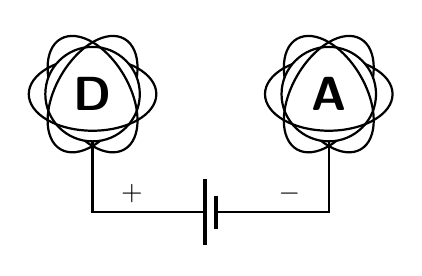
\begin{tikzpicture}
    % -----------------------------
    % Parameters (tweak as needed)
    % -----------------------------
    \def\R{.6 * 1.00}        % nucleus radius (cm)
    \def\ra{.6 * 2.70/2}     % orbit ellipse x-radius (cm)  = a
    \def\rb{.6 * 1.55/2}     % orbit ellipse y-radius (cm)  = b
    \def\lw{0.8pt}      % line width (uniform)
    \def\wireLen{2.3}   % length of the downward wire (cm)

    % Orbit rotation angles (degrees)
    \def\phiA{0}
    \def\phiB{60}
    \def\phiC{-60}

    % Label font for the nucleus text — adjust to taste
    \newcommand{\labelfont}{\sffamily\bfseries\fontsize{16pt}{16pt}\selectfont}
    % Try 18–28pt depending on how full you want the A to look relative to R=1cm.

    %-----------------------------
    % Styles and helpers
    % -----------------------------
    \tikzset{schem/.style={draw=black, line width=\lw, line cap=round, line join=round}}

    % Compute crossing angle θ× (degrees) for ellipse-circle intersection:
    % a^2 cos^2 t + b^2 sin^2 t = R^2  =>  cos^2 t = (R^2 - b^2)/(a^2 - b^2)
    % Clamp to [0,1] to avoid NaN if parameters are borderline.
    \pgfmathsetmacro{\coscrit}{(\R*\R - \rb*\rb)/(\ra*\ra - \rb*\rb)}
    \pgfmathsetmacro{\coscrit}{max(0,min(1,\coscrit))}
    \pgfmathsetmacro{\tCross}{acos(sqrt(\coscrit))}   % in degrees
    \pgfmathsetmacro{\tUpperStart}{\tCross}
    \pgfmathsetmacro{\tUpperEnd}{180 - \tCross}
    \pgfmathsetmacro{\tLowerStart}{-180 + \tCross}
    \pgfmathsetmacro{\tLowerEnd}{-\tCross}

    % Draw the single front arc (upper half inside the circle) for an ellipse rotated by φ
    \newcommand{\frontarcUpper}[3]{%
      \begin{scope}[shift={(#2,#3)},rotate=#1]
        \draw[schem] ({\ra*cos(\tUpperStart)},{\rb*sin(\tUpperStart)})
          arc[x radius=\ra, y radius=\rb,
              start angle=\tUpperStart, end angle=\tUpperEnd];
      \end{scope}
    }

    % Alternate: lower half inside the circle
    \newcommand{\frontarcLower}[3]{%
      \begin{scope}[shift={(#2,#3)},rotate=#1]
        \draw[schem] ({\ra*cos(\tLowerStart)},{\rb*sin(\tLowerStart)})
          arc[x radius=\ra, y radius=\rb,
              start angle=\tLowerStart, end angle=\tLowerEnd];
      \end{scope}
    }

  % Define variables for better adjustability
  \def\atomSep{3}         % Separation between atoms (horizontal distance)
  \def\rowSep{1.5}        % Base vertical spacing unit
  \def\batteryWidth{2}    % Width of the battery
    % Place the atoms (D for donor, A for acceptor)
    % These will be covered; just to provide origins for the circuit
    \node (D) at (0,0) {\labelfont D};
    \node (A) at (\atomSep,0) {\labelfont A};
    % -----------------------------
    % Full orbits (behind the nucleus)
    % -----------------------------
    \draw[schem] (0,0) ellipse [x radius=\ra, y radius=\rb, rotate=\phiA];
    \draw[schem] (0,0) ellipse [x radius=\ra, y radius=\rb, rotate=\phiB];
    \draw[schem] (0,0) ellipse [x radius=\ra, y radius=\rb, rotate=\phiC];
    \draw[schem] (\atomSep,0) ellipse [x radius=\ra, y radius=\rb, rotate=\phiA];
    \draw[schem] (\atomSep,0) ellipse [x radius=\ra, y radius=\rb, rotate=\phiB];
    \draw[schem] (\atomSep,0) ellipse [x radius=\ra, y radius=\rb, rotate=\phiC];
    % Battery placement
    \coordinate (BatLeft) at  (\atomSep/2 - \batteryWidth/2, -\rowSep);
    \coordinate (BatRight) at (\atomSep/2 + \batteryWidth/2, -\rowSep);

    % Draw the battery
    \draw[thick] (BatLeft) to[battery1, name=Bat] (BatRight);

    % Add + and - labels above battery terminals
    \node[above] at (BatLeft)  {$+$};
    \node[above] at (BatRight) {$-$};

    % Connect atoms to battery terminals
    \draw[thick] (D) |- (BatLeft);
    \draw[thick] (A) |- (BatRight);
    % -----------------------------
    % White disk to hide crossings (puts the mid-portion "behind")
    % -----------------------------
    \fill[white] (0,0) circle[radius=\R];
    \fill[white] (\atomSep,0) circle[radius=\R];

    % Place the atoms again, this time visibly
    \node at (0,0) {\labelfont D};
    \node at (\atomSep,0) {\labelfont A};

    % -----------------------------
    % One *front* arc per orbit (choose Upper/Lower per orbit)
    % -----------------------------
    \frontarcLower{\phiA}{0}{0}
    \frontarcUpper{\phiB}{0}{0}
    \frontarcUpper{\phiC}{0}{0}
    \frontarcLower{\phiA}{\atomSep}{0}
    \frontarcUpper{\phiB}{\atomSep}{0}
    \frontarcUpper{\phiC}{\atomSep}{0}

    % -----------------------------
    % Nucleus outline LAST to cover any seam
    % -----------------------------
    \draw[schem] (0,0) circle[radius=\R];
    \draw[schem] (\atomSep,0) circle[radius=\R];

\end{tikzpicture}
\end{document}

